% Options for packages loaded elsewhere
\PassOptionsToPackage{unicode}{hyperref}
\PassOptionsToPackage{hyphens}{url}
%
\documentclass[
  ignorenonframetext,
]{beamer}
\usepackage{pgfpages}
\setbeamertemplate{caption}[numbered]
\setbeamertemplate{caption label separator}{: }
\setbeamercolor{caption name}{fg=normal text.fg}
\beamertemplatenavigationsymbolsempty
% Prevent slide breaks in the middle of a paragraph
\widowpenalties 1 10000
\raggedbottom
\setbeamertemplate{part page}{
  \centering
  \begin{beamercolorbox}[sep=16pt,center]{part title}
    \usebeamerfont{part title}\insertpart\par
  \end{beamercolorbox}
}
\setbeamertemplate{section page}{
  \centering
  \begin{beamercolorbox}[sep=12pt,center]{part title}
    \usebeamerfont{section title}\insertsection\par
  \end{beamercolorbox}
}
\setbeamertemplate{subsection page}{
  \centering
  \begin{beamercolorbox}[sep=8pt,center]{part title}
    \usebeamerfont{subsection title}\insertsubsection\par
  \end{beamercolorbox}
}
\AtBeginPart{
  \frame{\partpage}
}
\AtBeginSection{
  \ifbibliography
  \else
    \frame{\sectionpage}
  \fi
}
\AtBeginSubsection{
  \frame{\subsectionpage}
}
\usepackage{amsmath,amssymb}
\usepackage{lmodern}
\usepackage{ifxetex,ifluatex}
\ifnum 0\ifxetex 1\fi\ifluatex 1\fi=0 % if pdftex
  \usepackage[T1]{fontenc}
  \usepackage[utf8]{inputenc}
  \usepackage{textcomp} % provide euro and other symbols
\else % if luatex or xetex
  \usepackage{unicode-math}
  \defaultfontfeatures{Scale=MatchLowercase}
  \defaultfontfeatures[\rmfamily]{Ligatures=TeX,Scale=1}
  \setmainfont[BoldFont = SF Pro Rounded Semibold]{SF Pro Rounded}
  \setmathfont[]{STIX Two Math}
\fi
\usefonttheme{serif} % use mainfont rather than sansfont for slide text
% Use upquote if available, for straight quotes in verbatim environments
\IfFileExists{upquote.sty}{\usepackage{upquote}}{}
\IfFileExists{microtype.sty}{% use microtype if available
  \usepackage[]{microtype}
  \UseMicrotypeSet[protrusion]{basicmath} % disable protrusion for tt fonts
}{}
\makeatletter
\@ifundefined{KOMAClassName}{% if non-KOMA class
  \IfFileExists{parskip.sty}{%
    \usepackage{parskip}
  }{% else
    \setlength{\parindent}{0pt}
    \setlength{\parskip}{6pt plus 2pt minus 1pt}}
}{% if KOMA class
  \KOMAoptions{parskip=half}}
\makeatother
\usepackage{xcolor}
\IfFileExists{xurl.sty}{\usepackage{xurl}}{} % add URL line breaks if available
\IfFileExists{bookmark.sty}{\usepackage{bookmark}}{\usepackage{hyperref}}
\hypersetup{
  pdftitle={444 Lecture 3.3 - Backward Induction and Ties},
  pdfauthor={Brian Weatherson},
  hidelinks,
  pdfcreator={LaTeX via pandoc}}
\urlstyle{same} % disable monospaced font for URLs
\newif\ifbibliography
\usepackage{graphicx}
\makeatletter
\def\maxwidth{\ifdim\Gin@nat@width>\linewidth\linewidth\else\Gin@nat@width\fi}
\def\maxheight{\ifdim\Gin@nat@height>\textheight\textheight\else\Gin@nat@height\fi}
\makeatother
% Scale images if necessary, so that they will not overflow the page
% margins by default, and it is still possible to overwrite the defaults
% using explicit options in \includegraphics[width, height, ...]{}
\setkeys{Gin}{width=\maxwidth,height=\maxheight,keepaspectratio}
% Set default figure placement to htbp
\makeatletter
\def\fps@figure{htbp}
\makeatother
\setlength{\emergencystretch}{3em} % prevent overfull lines
\providecommand{\tightlist}{%
  \setlength{\itemsep}{0pt}\setlength{\parskip}{0pt}}
\setcounter{secnumdepth}{-\maxdimen} % remove section numbering
\let\Tiny=\tiny

 \setbeamertemplate{navigation symbols}{} 

% \usetheme{Madrid}
 \usetheme[numbering=none, progressbar=foot]{metropolis}
 \usecolortheme{wolverine}
 \usepackage{color}
 \usepackage{MnSymbol}
% \usepackage{movie15}

\usepackage{amssymb}% http://ctan.org/pkg/amssymb
\usepackage{pifont}% http://ctan.org/pkg/pifont
\newcommand{\cmark}{\ding{51}}%
\newcommand{\xmark}{\ding{55}}%

\DeclareSymbolFont{symbolsC}{U}{txsyc}{m}{n}
\DeclareMathSymbol{\boxright}{\mathrel}{symbolsC}{128}
\DeclareMathAlphabet{\mathpzc}{OT1}{pzc}{m}{it}

\setlength{\parskip}{1ex plus 0.5ex minus 0.2ex}

\AtBeginSection[]
{
\begin{frame}
	\Huge{\color{darkblue} \insertsection}
\end{frame}
}

\renewenvironment*{quote}	
	{\list{}{\rightmargin   \leftmargin} \item } 	
	{\endlist }

\definecolor{darkgreen}{rgb}{0,0.7,0}
\definecolor{darkblue}{rgb}{0,0,0.8}

\usepackage[italic]{mathastext}
\usepackage{nicefrac}

\setbeamertemplate{caption}{\raggedright\insertcaption}

%\def\toprule{}
%\def\bottomrule{}
%\def\midrule{}
\usepackage{etoolbox}
\AfterEndEnvironment{description}{\vspace{9pt}}
\AfterEndEnvironment{oltableau}{\vspace{9pt}}
\BeforeBeginEnvironment{oltableau}{\vspace{9pt}}
\AfterEndEnvironment{center}{\vspace{9pt}}
\BeforeBeginEnvironment{tabular}{\vspace{9pt}}
\AfterEndEnvironment{longtable}{\vspace{-6pt}}
\usepackage{booktabs}
\usepackage{longtable}
\usepackage{array}
\usepackage{multirow}
\usepackage{wrapfig}
\usepackage{float}
\usepackage{colortbl}
\usepackage{pdflscape}
\usepackage{tabu}
\usepackage{threeparttable} 
\usepackage{threeparttablex} 
\usepackage[normalem]{ulem} 
\usepackage{makecell}
\usepackage{xcolor}
\usepackage{ulem}

\setlength\heavyrulewidth{0ex}
\setlength\lightrulewidth{0.08ex}

\aboverulesep=0ex
\belowrulesep=0ex
\renewcommand{\arraystretch}{1.2}
\ifluatex
  \usepackage{selnolig}  % disable illegal ligatures
\fi

\title{444 Lecture 3.3 - Backward Induction and Ties}
\author{Brian Weatherson}
\date{}

\begin{document}
\frame{\titlepage}

\begin{frame}{Plan}
\protect\hypertarget{plan}{}
To address a bug in the backwards induction algorithm - ties.
\end{frame}

\begin{frame}{Reading}
\protect\hypertarget{reading}{}
Bonanno, section 3.2.
\end{frame}

\begin{frame}{Backwards Induction in Positive Sum Games}
\protect\hypertarget{backwards-induction-in-positive-sum-games}{}
\begin{figure}
\centering
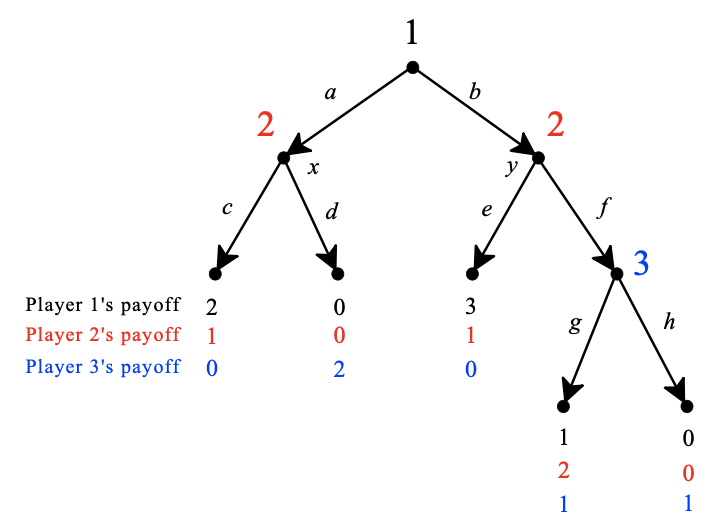
\includegraphics[width=\textwidth,height=0.6\textheight]{images/3_3a.png}
\caption{Three player game tree}
\end{figure}

\begin{itemize}
\tightlist
\item
  This is three player, but crucially, it is not zero sum.
\end{itemize}
\end{frame}

\begin{frame}
\begin{figure}
\centering
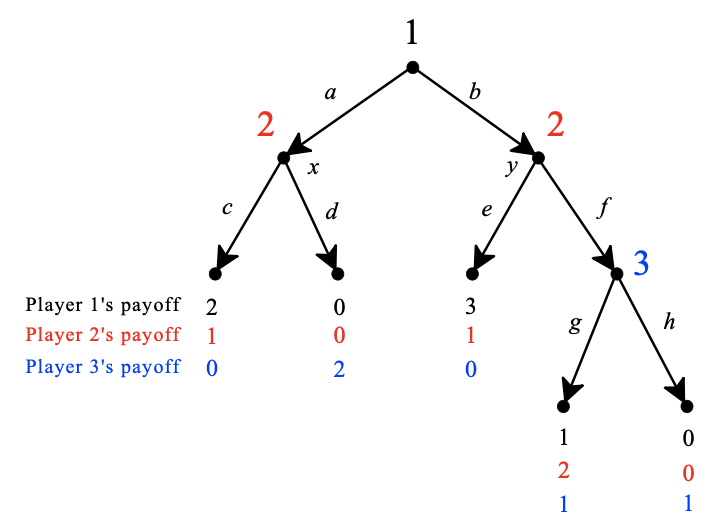
\includegraphics[width=\textwidth,height=0.6\textheight]{images/3_3a.png}
\caption{Three player game tree}
\end{figure}

\begin{itemize}[<+->]
\tightlist
\item
  In the bottom right, Player 3 doesn't care which choice is made.
\item
  So we can't infer what Player 3 will do.
\end{itemize}
\end{frame}

\begin{frame}
\begin{figure}
\centering
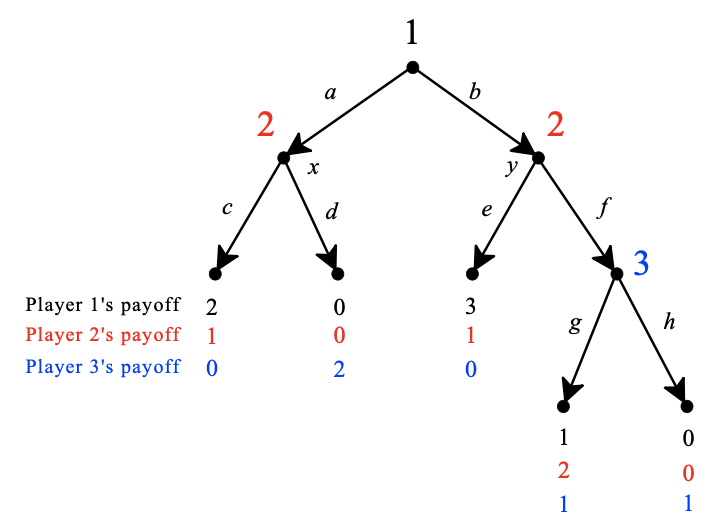
\includegraphics[width=\textwidth,height=0.6\textheight]{images/3_3a.png}
\caption{Three player game tree}
\end{figure}

\begin{itemize}[<+->]
\tightlist
\item
  But the other players do care what Player 3 will do.
\item
  So we can't just ignore this choice.
\end{itemize}
\end{frame}

\begin{frame}
\begin{figure}
\centering
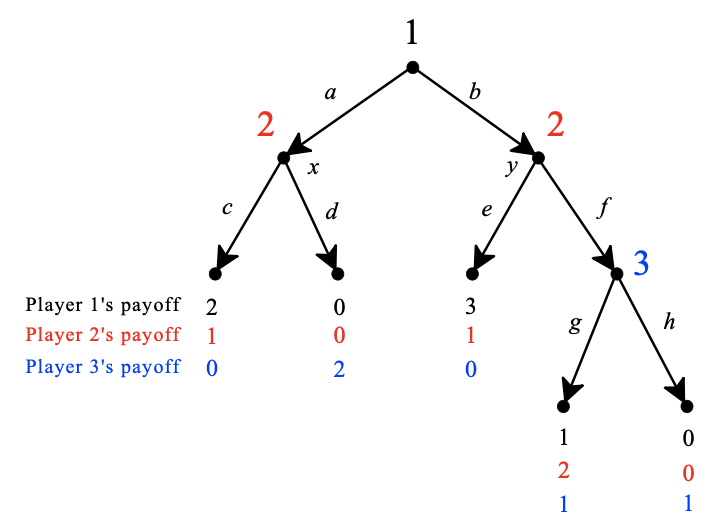
\includegraphics[width=\textwidth,height=0.6\textheight]{images/3_3a.png}
\caption{Three player game tree}
\end{figure}

\begin{itemize}
\tightlist
\item
  The solution is to build two trees, one for each of Player 3's
  choices.
\end{itemize}
\end{frame}

\begin{frame}
\begin{figure}
\centering
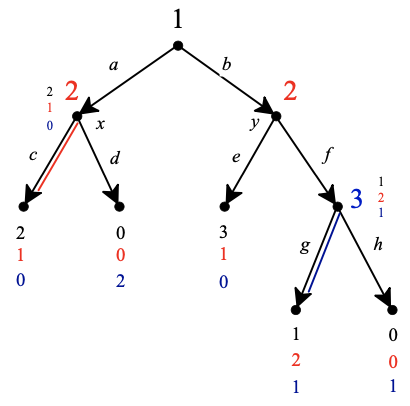
\includegraphics[width=\textwidth,height=0.6\textheight]{images/3_3b.png}
\caption{Solution One}
\end{figure}

\begin{itemize}
\tightlist
\item
  First, assume 3 plays g.
\item
  Then 2 would play f at node y.
\item
  So 1 will actually play a.
\end{itemize}
\end{frame}

\begin{frame}
\begin{figure}
\centering
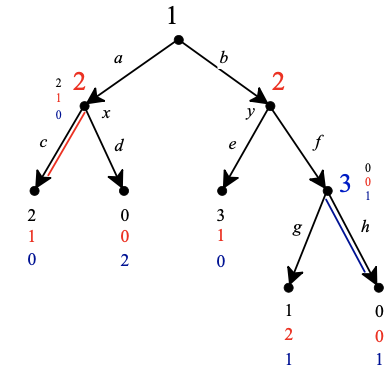
\includegraphics[width=\textwidth,height=0.6\textheight]{images/3_3c.png}
\caption{Solution One}
\end{figure}

\begin{itemize}
\tightlist
\item
  Now, assume 3 plays h.
\item
  Then 2 would play e at node y.
\item
  So 1 will actually play b triggering this play.
\end{itemize}
\end{frame}

\begin{frame}{Multiple Solutions}
\protect\hypertarget{multiple-solutions}{}
\begin{itemize}
\tightlist
\item
  This is a game with multiple backwards induction solutions.
\item
  The solutions don't just differ in what Player 3, who faces the tie,
  plays.
\item
  They differ in the very first move!
\item
  This is the totally general case; most solution concepts are like
  this.
\item
  But it's a pain to deal with.
\end{itemize}
\end{frame}

\begin{frame}{For Next Time}
\protect\hypertarget{for-next-time}{}
\begin{itemize}
\tightlist
\item
  We will look at how game trees relate to what we did last week.
\end{itemize}
\end{frame}

\end{document}
